\documentclass[12pt]{article}
%Fall 2022
% Some basic packages
\usepackage{standalone}[subpreambles=true]
\usepackage[utf8]{inputenc}
\usepackage[T1]{fontenc}
\usepackage{textcomp}
\usepackage[english]{babel}
\usepackage{url}
\usepackage{graphicx}
%\usepackage{quiver}
\usepackage{float}
\usepackage{enumitem}
\usepackage{lmodern}
\usepackage{comment}
\usepackage{hyperref}
\usepackage[usenames,svgnames,dvipsnames]{xcolor}
\usepackage[margin=1in]{geometry}
\usepackage{pdfpages}

\pdfminorversion=7

% Don't indent paragraphs, leave some space between them
\usepackage{parskip}

% Hide page number when page is empty
\usepackage{emptypage}
\usepackage{subcaption}
\usepackage{multicol}
\usepackage[b]{esvect}

% Math stuff
\usepackage{amsmath, amsfonts, mathtools, amsthm, amssymb}
\usepackage{bbm}
\usepackage{stmaryrd}
\allowdisplaybreaks

% Fancy script capitals
\usepackage{mathrsfs}
\usepackage{cancel}
% Bold math
\usepackage{bm}
% Some shortcuts
\newcommand{\rr}{\ensuremath{\mathbb{R}}}
\newcommand{\zz}{\ensuremath{\mathbb{Z}}}
\newcommand{\qq}{\ensuremath{\mathbb{Q}}}
\newcommand{\nn}{\ensuremath{\mathbb{N}}}
\newcommand{\ff}{\ensuremath{\mathbb{F}}}
\newcommand{\cc}{\ensuremath{\mathbb{C}}}
\newcommand{\ee}{\ensuremath{\mathbb{E}}}
\newcommand{\hh}{\ensuremath{\mathbb{H}}}
\renewcommand\O{\ensuremath{\emptyset}}
\newcommand{\norm}[1]{{\left\lVert{#1}\right\rVert}}
\newcommand{\dbracket}[1]{{\left\llbracket{#1}\right\rrbracket}}
\newcommand{\ve}[1]{{\bm{#1}}}
\newcommand\allbold[1]{{\boldmath\textbf{#1}}}
\DeclareMathOperator{\lcm}{lcm}
\DeclareMathOperator{\im}{im}
\DeclareMathOperator{\coim}{coim}
\DeclareMathOperator{\dom}{dom}
\DeclareMathOperator{\tr}{tr}
\DeclareMathOperator{\rank}{rank}
\DeclareMathOperator*{\var}{Var}
\DeclareMathOperator*{\ev}{E}
\DeclareMathOperator{\dg}{deg}
\DeclareMathOperator{\aff}{aff}
\DeclareMathOperator{\conv}{conv}
\DeclareMathOperator{\inte}{int}
\DeclareMathOperator*{\argmin}{argmin}
\DeclareMathOperator*{\argmax}{argmax}
\DeclareMathOperator{\graph}{graph}
\DeclareMathOperator{\sgn}{sgn}
\DeclareMathOperator*{\Rep}{Rep}
\DeclareMathOperator{\Proj}{Proj}
\DeclareMathOperator{\mat}{mat}
\DeclareMathOperator{\diag}{diag}
\DeclareMathOperator{\aut}{Aut}
\DeclareMathOperator{\gal}{Gal}
\DeclareMathOperator{\inn}{Inn}
\DeclareMathOperator{\edm}{End}
\DeclareMathOperator{\Hom}{Hom}
\DeclareMathOperator{\ext}{Ext}
\DeclareMathOperator{\tor}{Tor}
\DeclareMathOperator{\Span}{Span}
\DeclareMathOperator{\Stab}{Stab}
\DeclareMathOperator{\cont}{cont}
\DeclareMathOperator{\Ann}{Ann}
\DeclareMathOperator{\Div}{div}
\DeclareMathOperator{\curl}{curl}
\DeclareMathOperator{\nat}{Nat}
\DeclareMathOperator{\gr}{Gr}
\DeclareMathOperator{\vect}{Vect}
\DeclareMathOperator{\id}{id}
\DeclareMathOperator{\Mod}{Mod}
\DeclareMathOperator{\sign}{sign}
\DeclareMathOperator{\Surf}{Surf}
\DeclareMathOperator{\fcone}{fcone}
\DeclareMathOperator{\Rot}{Rot}
\DeclareMathOperator{\grad}{grad}
\DeclareMathOperator{\atan2}{atan2}
\DeclareMathOperator{\Ric}{Ric}
\let\vec\relax
\DeclareMathOperator{\vec}{vec}
\let\Re\relax
\DeclareMathOperator{\Re}{Re}
\let\Im\relax
\DeclareMathOperator{\Im}{Im}
% Put x \to \infty below \lim
\let\svlim\lim\def\lim{\svlim\limits}

%wide hat
\usepackage{scalerel,stackengine}
\stackMath
\newcommand*\wh[1]{%
\savestack{\tmpbox}{\stretchto{%
  \scaleto{%
    \scalerel*[\widthof{\ensuremath{#1}}]{\kern-.6pt\bigwedge\kern-.6pt}%
    {\rule[-\textheight/2]{1ex}{\textheight}}%WIDTH-LIMITED BIG WEDGE
  }{\textheight}% 
}{0.5ex}}%
\stackon[1pt]{#1}{\tmpbox}%
}
\parskip 1ex

%Make implies and impliedby shorter
\let\implies\Rightarrow
\let\impliedby\Leftarrow
\let\iff\Leftrightarrow
\let\epsilon\varepsilon

% Add \contra symbol to denote contradiction
\usepackage{stmaryrd} % for \lightning
\newcommand\contra{\scalebox{1.5}{$\lightning$}}

% \let\phi\varphi

% Command for short corrections
% Usage: 1+1=\correct{3}{2}

\definecolor{correct}{HTML}{009900}
\newcommand\correct[2]{\ensuremath{\:}{\color{red}{#1}}\ensuremath{\to }{\color{correct}{#2}}\ensuremath{\:}}
\newcommand\green[1]{{\color{correct}{#1}}}

% horizontal rule
\newcommand\hr{
    \noindent\rule[0.5ex]{\linewidth}{0.5pt}
}

% hide parts
\newcommand\hide[1]{}

% si unitx
\usepackage{siunitx}
\sisetup{locale = FR}

%allows pmatrix to stretch
\makeatletter
\renewcommand*\env@matrix[1][\arraystretch]{%
  \edef\arraystretch{#1}%
  \hskip -\arraycolsep
  \let\@ifnextchar\new@ifnextchar
  \array{*\c@MaxMatrixCols c}}
\makeatother

\renewcommand{\arraystretch}{0.8}

\renewcommand{\baselinestretch}{1.5}

\usepackage{graphics}
\usepackage{epstopdf}

\RequirePackage{hyperref}
%%
%% Add support for color in order to color the hyperlinks.
%% 
\hypersetup{
  colorlinks = true,
  urlcolor = blue,
  citecolor = blue
}
%%fakesection Links
\hypersetup{
    colorlinks,
    linkcolor={red!50!black},
    citecolor={green!50!black},
    urlcolor={blue!80!black}
}
%customization of cleveref
\RequirePackage[capitalize,nameinlink]{cleveref}[0.19]

% Per SIAM Style Manual, "section" should be lowercase
\crefname{section}{section}{sections}
\crefname{subsection}{subsection}{subsections}
\Crefname{section}{Section}{Sections}
\Crefname{subsection}{Subsection}{Subsections}

% Per SIAM Style Manual, "Figure" should be spelled out in references
\Crefname{figure}{Figure}{Figures}

% Per SIAM Style Manual, don't say equation in front on an equation.
\crefformat{equation}{\textup{#2(#1)#3}}
\crefrangeformat{equation}{\textup{#3(#1)#4--#5(#2)#6}}
\crefmultiformat{equation}{\textup{#2(#1)#3}}{ and \textup{#2(#1)#3}}
{, \textup{#2(#1)#3}}{, and \textup{#2(#1)#3}}
\crefrangemultiformat{equation}{\textup{#3(#1)#4--#5(#2)#6}}%
{ and \textup{#3(#1)#4--#5(#2)#6}}{, \textup{#3(#1)#4--#5(#2)#6}}{, and \textup{#3(#1)#4--#5(#2)#6}}

% But spell it out at the beginning of a sentence.
\Crefformat{equation}{#2Equation~\textup{(#1)}#3}
\Crefrangeformat{equation}{Equations~\textup{#3(#1)#4--#5(#2)#6}}
\Crefmultiformat{equation}{Equations~\textup{#2(#1)#3}}{ and \textup{#2(#1)#3}}
{, \textup{#2(#1)#3}}{, and \textup{#2(#1)#3}}
\Crefrangemultiformat{equation}{Equations~\textup{#3(#1)#4--#5(#2)#6}}%
{ and \textup{#3(#1)#4--#5(#2)#6}}{, \textup{#3(#1)#4--#5(#2)#6}}{, and \textup{#3(#1)#4--#5(#2)#6}}

% Make number non-italic in any environment.
\crefdefaultlabelformat{#2\textup{#1}#3}

% Environments
\makeatother
% For box around Definition, Theorem, \ldots
%%fakesection Theorems
\usepackage{thmtools}
\usepackage[framemethod=TikZ]{mdframed}

\theoremstyle{definition}
\mdfdefinestyle{mdbluebox}{%
	roundcorner = 10pt,
	linewidth=1pt,
	skipabove=12pt,
	innerbottommargin=9pt,
	skipbelow=2pt,
	nobreak=true,
	linecolor=blue,
	backgroundcolor=TealBlue!5,
}
\declaretheoremstyle[
	headfont=\sffamily\bfseries\color{MidnightBlue},
	mdframed={style=mdbluebox},
	headpunct={\\[3pt]},
	postheadspace={0pt}
]{thmbluebox}

\mdfdefinestyle{mdredbox}{%
	linewidth=0.5pt,
	skipabove=12pt,
	frametitleaboveskip=5pt,
	frametitlebelowskip=0pt,
	skipbelow=2pt,
	frametitlefont=\bfseries,
	innertopmargin=4pt,
	innerbottommargin=8pt,
	nobreak=false,
	linecolor=RawSienna,
	backgroundcolor=Salmon!5,
}
\declaretheoremstyle[
	headfont=\bfseries\color{RawSienna},
	mdframed={style=mdredbox},
	headpunct={\\[3pt]},
	postheadspace={0pt},
]{thmredbox}

\declaretheorem[%
style=thmbluebox,name=Theorem,numberwithin=section]{thm}
\declaretheorem[style=thmbluebox,name=Lemma,sibling=thm]{lem}
\declaretheorem[style=thmbluebox,name=Proposition,sibling=thm]{prop}
\declaretheorem[style=thmbluebox,name=Corollary,sibling=thm]{coro}
\declaretheorem[style=thmredbox,name=Example,sibling=thm]{eg}

\mdfdefinestyle{mdgreenbox}{%
	roundcorner = 10pt,
	linewidth=1pt,
	skipabove=12pt,
	innerbottommargin=9pt,
	skipbelow=2pt,
	nobreak=true,
	linecolor=ForestGreen,
	backgroundcolor=ForestGreen!5,
}

\declaretheoremstyle[
	headfont=\bfseries\sffamily\color{ForestGreen!70!black},
	bodyfont=\normalfont,
	spaceabove=2pt,
	spacebelow=1pt,
	mdframed={style=mdgreenbox},
	headpunct={ --- },
]{thmgreenbox}

\declaretheorem[style=thmgreenbox,name=Definition,sibling=thm]{defn}

\mdfdefinestyle{mdgreenboxsq}{%
	linewidth=1pt,
	skipabove=12pt,
	innerbottommargin=9pt,
	skipbelow=2pt,
	nobreak=true,
	linecolor=ForestGreen,
	backgroundcolor=ForestGreen!5,
}
\declaretheoremstyle[
	headfont=\bfseries\sffamily\color{ForestGreen!70!black},
	bodyfont=\normalfont,
	spaceabove=2pt,
	spacebelow=1pt,
	mdframed={style=mdgreenboxsq},
	headpunct={},
]{thmgreenboxsq}
\declaretheoremstyle[
	headfont=\bfseries\sffamily\color{ForestGreen!70!black},
	bodyfont=\normalfont,
	spaceabove=2pt,
	spacebelow=1pt,
	mdframed={style=mdgreenboxsq},
	headpunct={},
]{thmgreenboxsq*}

\mdfdefinestyle{mdblackbox}{%
	skipabove=8pt,
	linewidth=3pt,
	rightline=false,
	leftline=true,
	topline=false,
	bottomline=false,
	linecolor=black,
	backgroundcolor=RedViolet!5!gray!5,
}
\declaretheoremstyle[
	headfont=\bfseries,
	bodyfont=\normalfont\small,
	spaceabove=0pt,
	spacebelow=0pt,
	mdframed={style=mdblackbox}
]{thmblackbox}

\theoremstyle{plain}
\declaretheorem[name=Question,sibling=thm,style=thmblackbox]{ques}
\declaretheorem[name=Remark,sibling=thm,style=thmgreenboxsq]{remark}
\declaretheorem[name=Remark,sibling=thm,style=thmgreenboxsq*]{remark*}
\newtheorem{ass}[thm]{Assumptions}

\theoremstyle{definition}
\newtheorem*{problem}{Problem}
\newtheorem{claim}[thm]{Claim}
\theoremstyle{remark}
\newtheorem*{case}{Case}
\newtheorem*{notation}{Notation}
\newtheorem*{note}{Note}
\newtheorem*{motivation}{Motivation}
\newtheorem*{intuition}{Intuition}
\newtheorem*{conjecture}{Conjecture}

% Make section starts with 1 for report type
%\renewcommand\thesection{\arabic{section}}

% End example and intermezzo environments with a small diamond (just like proof
% environments end with a small square)
\usepackage{etoolbox}
\AtEndEnvironment{vb}{\null\hfill$\diamond$}%
\AtEndEnvironment{intermezzo}{\null\hfill$\diamond$}%
% \AtEndEnvironment{opmerking}{\null\hfill$\diamond$}%

% Fix some spacing
% http://tex.stackexchange.com/questions/22119/how-can-i-change-the-spacing-before-theorems-with-amsthm
\makeatletter
\def\thm@space@setup{%
  \thm@preskip=\parskip \thm@postskip=0pt
}

% Fix some stuff
% %http://tex.stackexchange.com/questions/76273/multiple-pdfs-with-page-group-included-in-a-single-page-warning
\pdfsuppresswarningpagegroup=1


% My name
\author{Jaden Wang}



\begin{document}
\centerline {\textsf{\textbf{\LARGE{Satellite Attitude Dynamics Simuation Report}}}}
\centerline {Jaden Wang}

Consider the problem of a 3D rigid body rotating freely in space. We assume that there are no external torque or force so the angular momentum and total energy are conserved. Let $ P_t$ be the body frame consisting of three unit length principal axes of the object at time $ t$ and without loss of generality assume the inertia frame coincides with the principal axes at time $ t_0$, \emph{i.e.} $ P_0 = I$. Let $ \omega(t)$ be the angular velocity of the object as a function of time. Since it is most convenient to use the moment of inertia $ \mathcal{ I}$ in the body frame, $ \omega$ should also be expressed using the principal axes coordinates.
\section{Kinematic equations}
Euler's 2nd law states
\begin{align*}
	\sum M^{C} = \frac{\ ^IdH^{C}}{ dt} = \frac{\ ^BdH^{C}}{ dt} + \ ^I \omega^{B} \times H^{C} .
\end{align*}
Thus in the body frame, we have
\begin{align*}
	0=M_{net} &= \mathcal{ I} \dot{\omega} + \widetilde{ \omega} \mathcal{ I} \omega \\
	\dot{\omega} &= -\mathcal{ I}^{-1} (\widetilde{ \omega} \mathcal{ I} \omega ),
\end{align*}
where $ \widetilde{ \omega}$ is the dual matrix of $ \omega$. This yields 3 Euler kinematics equations.
\subsection{Direction cosine matrix}
The DCM$\ ^AC^B \in SO(3)$ relates the coordinates of any vector $ v$ in inertial frame to those in the body frame in the following way:
\begin{align*}
	\ ^Av = \ ^AC^B \ ^Bv  .
\end{align*}
Since it is most convenient to use the moment of inertia $ \mathcal{ I}$ in the body frame,  To convert it back to the inertia frame, we need to apply $ C:= \ ^AC^B$. Then this yields the 9 Poisson kinematics equations:
\begin{align*}
	\dot{C} = C \widetilde{ \omega}.
\end{align*}
Together we have a system of 12 differential equations.
\subsection{Euler angles}
We can decompose a rotation into three simple rotations about each principal axis, which can be fully described by three angles $ (\theta,\phi,\psi) \in S^{1}\times S^{1} \times S^{1} =:T^{3}$, the 3-torus. However, each time we perform a simple rotation, the inertial coordinates of the principal axes change. By the addition theorem, we can express $ \omega$ using a mixed basis
\begin{align*}
	\ ^A\omega^B &= \ ^A \omega^{B'} + \ ^{B'} \omega^{B''} + \ ^{B''} \omega^{B} \\
	&= \dot{\theta} \wh{ b}_1' + \dot{\phi} \wh{ b}_2'' + \dot{\psi} \wh{ b}_3\\
	&= \omega_1 \wh{ b}_1 + \omega_2 \wh{ b}_2 + \omega_3 \wh{ b}_3 
\end{align*}
We can find the matrix that relates the mixed basis with the body frame and obtain
\begin{align*}
	\omega = \begin{pmatrix} c_2 c_3 & s_3 & 0\\ -c_2s_3 & c_3 &0\\ s_2&0&1 \end{pmatrix} \begin{pmatrix} \dot{\theta}\\ \dot{\phi}\\ \dot{\psi} \end{pmatrix} ,
\end{align*}
where $ c = \cos$, $ s= \sin$, and the indices correspond to $ (\theta,\phi,\psi)$. Therefore, as long as this matrix is invertible, we can obtain the necessary ODEs to solve the system by multiplying its inverse on both sides. However, the matrix clearly has a singularity if $ \phi = \psi = \frac{\pi}{2}$. This singularity is called gimbal lock. If you like topology, I included a math proof to show that gimbal lock is inevitable using only three angle parameters at the end of this report.

We can convert the three angles back to DCM $ C$ via the following formula:
 \begin{align*}
	 C = \begin{pmatrix} c_2c_3&-c_2s_3&s_2\\s_1s_2c_3+s_3c_1&-s_1s_2s_3+c_3c_1&-s_1 c_2\\ -c_1s_2c_3+s_3s_1&c_1s_2s_3+c_3s_1&c_1c_2 \end{pmatrix} .
\end{align*}
\subsection{Quarternions}
By Euler's theorem on rotation, we can represent any rotation in $ \rr^3$ by an unit vector $ \lambda$ and an angle $ \theta$. Now set
\begin{align*}
	\epsilon = \begin{pmatrix} \sin \frac{\theta}{2} \lambda \\ \cos \frac{\theta}{2} \end{pmatrix} 
\end{align*}
This is a unit vector. We have the following dynamics
\begin{align*}
	\dot{ \epsilon} = \frac{1}{2} \begin{pmatrix} \epsilon_4&- \epsilon_3& \epsilon_2& \epsilon_1 \\ \epsilon_3& \epsilon_4& - \epsilon_1 & \epsilon_2\\ - \epsilon_2 & \epsilon_1 & \epsilon_4 & \epsilon_3\\ - \epsilon_1& - \epsilon_2 & - \epsilon_3 & \epsilon_4 \end{pmatrix}  \begin{pmatrix} \omega_1\\ \omega_2 \\ \omega_3 \\0 \end{pmatrix} .
\end{align*}
We see that this matrix is orthogonal and thus always invertible. To convert to DCM $ C$, we have
 \begin{align*}
	C = (1- 2 \overline{ \epsilon}^{T} \overline{ \epsilon}) I + 2 \overline{ \epsilon} \overline{ \epsilon}^{T} + 2 \epsilon_4 \widetilde{ \overline{ \epsilon}},
\end{align*}
where $ \overline{ \epsilon}$ is the first three components of $ \epsilon$ and $ \widetilde{ \overline{ \epsilon}}$ is again the dual matrix.

\section{Verification of Three Methods}
We set $ \mathcal{ I} = \begin{pmatrix} 5&0&0\\0&3&0\\0&0&10 \end{pmatrix} $ so we can demonstrate the tennis racket theorem about the $ x$-axis. To keep things exciting, the initial $ \omega_0$ is random. The initial frame coincides with inertia $ x,y,z$ coordinates, which means that  $C_0 = I, (\theta,\phi,\psi) = (0,0,0),  \epsilon = (0,0,0,1)$.

We have the same initial conditions for all three methods. Therefore, all energy and angular momentum plots are nearly identical up to numerical errors. The plots suggested that energy and angular momentum are indeed conserved in all three methods! Further, I demonstrated the tennis racket theorem in my animation, further validating the result. 
~\begin{figure}[H]
	\centering
	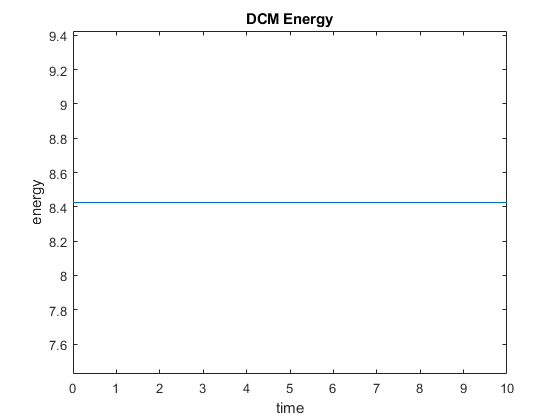
\includegraphics[width=0.49\textwidth]{./figures/sim2.1.png}
	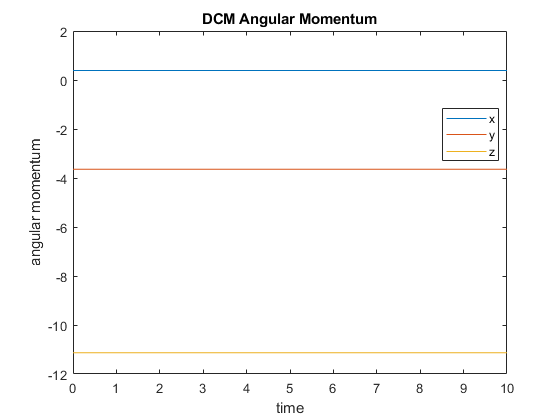
\includegraphics[width=0.49\textwidth]{./figures/sim2.2.png}
	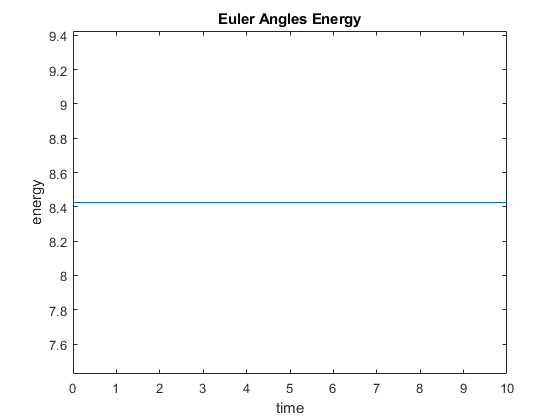
\includegraphics[width=0.49\textwidth]{./figures/sim2.3.png}
	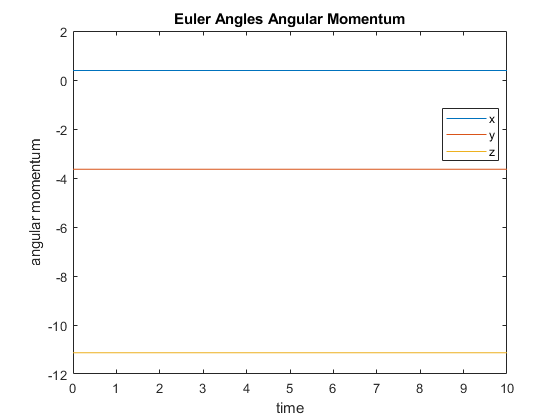
\includegraphics[width=0.49\textwidth]{./figures/sim2.4.png}
	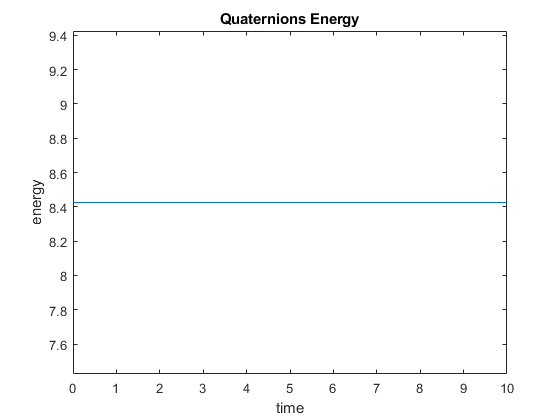
\includegraphics[width=0.49\textwidth]{./figures/sim2.5.png}
	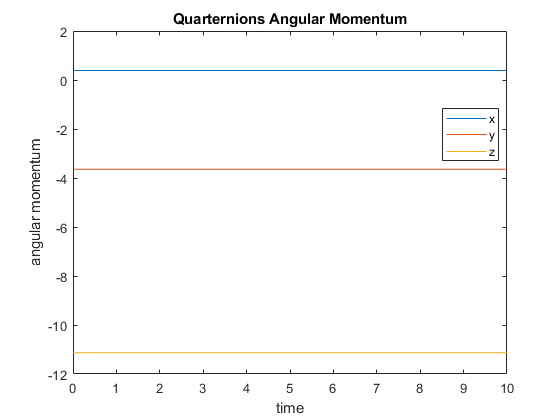
\includegraphics[width=0.49\textwidth]{./figures/sim2.6.png}
\end{figure}

\section{Comparisons}
Since $ \textsf{ODE89}$ doesn't allow me to specific fixed time steps, it is invalid to compare the accuracy of methods using standard deviations as methods with most numerical issues have more time steps and therefore reduced variance. The only valid metric I can think of is using the number of time steps, since fewer time steps mean that the desired numerical accuracy is achieved without trying too hard so the method is more accurate. In this run, we see that quarternions used 257 time steps, DMC used 297 time steps, and Euler angles used 377 time steps. Thus it appears that quarternions is the most numerically accurate method, whereas Euler angle is the least. This matches our expectations since Euler angle can give ill-conditioned matrices that we have to invert, but the quarternions require no inversion since the inverse is just the transpose. DCM might suffer slightly from not remaining entirely orthogonal due to numerical errors.
\section{A math proof of gimbal lock}

I want to present a super cool mathematical proof that gimbal lock will always occur when using three angles regardless of how clever we are. First, we can show that as smooth manifolds $ SO(3) \cong \rr P^3$, the real projective 3-space. This is essentially Euler's theorem on rotation: any rotation in $ \rr^3$ can be realized by rotating about a single oriented axis $ v$ which we can represent by an unit vector. Thus the set of axes of rotations gives us the unit sphere $ S^2$. The angle can be chosen from $ [0,\pi]$ since we can use $ -v$ as axis to cover  $ 2\pi$ rotation. Then rotations can be determined by elements of $ S^2 \times [0,\pi]$ (not uniquely). Moreover, zero rotation can be achieved by any axis, so we quotient out $ S^2\times \{0\}$. Notice that $ S^2 \times [0, \pi] / S^2 \times \{0\} $ can be thought of as a 3-ball with radius $ \pi$ since the hole at $ 0$ in the thickened sphere is now filled. Since rotating about $ v$ by $ \pi$ and $ -v$ by $\pi$ gives the same rotation, we can quotient them out by identifying antipodal points on the boundary of the 3-ball, thus obtaining $ \rr P^3$. There are no more ways to get the same rotation using different equivalence classes, so we achieved the bijection and can easily show they are diffeomorphic.

Now the question becomes, can we map the derivatives on $ T^3$ to derivatives on $ \rr P^3$ in an invertible way? Formally, suppose there exists a smooth map $f: T^3 \to \rr P^3$ s.t.\ its derivative $ df_p: T_pT^3 \to T_{f(p)} \rr P^3$ is invertible for every $ p \in T^3$. By inverse function theorem, $ f$ is therefore a local diffeomorphism. Now since  $ T^3$ and $ \rr P^3$ are Hausdorff, compact, and connected, by \href{https://math.stackexchange.com/questions/45990/when-is-a-local-homeomorphism-a-covering-map?lq=1}{some point-set topology argument}, $ f$ must be a covering map. But that implies that $ T^3$ is a covering space of $ \rr P^3$. This cannot be true, since the fundamental group of $ \pi_1(T^3) = \zz^3$ yet $ \pi_1(\rr P^3) = \zz /2$, but by covering space theory, $ \pi_1(T^3)$ should be a subgroup of $ \pi_1( \rr P^3)$, which is clearly impossible. Thus we establish that we cannot have any smooth map that avoids singularities in this situation!

\end{document}
